\documentclass[../main.tex]{subfiles}

\makeatletter
\@ifundefined{fromRoot}{%
  \newcommand{\fromRoot}[1]{../#1}
  
 % \usepackage{xr}
  % \externaldocument{../main}
}{}

\def\input@path{{\subfix{../}}}
%or: \def\input@path{{/path/to/folder/}{/path/to/other/folder/}}
\makeatother

\graphicspath{
  {\subfix{../}}
  {\subfix{./figures}}
  {\subfix{../figures}}
  {\subfix{./figures/logos-thesis/}}
  {\subfix{../figures/logos-thesis/}}
  {\subfix{./figures/rtexps-pics/}}
  {\subfix{../figures/rtexps-pics/}}
}

\hypersetup{
    pdfauthor   = {Camille MONIÈRE},
    pdftitle    = {Th\`{e}se (Présentation: expériences grandeur-natures)},
    pdfsubject  = {Th\`{e}se (Présentation: expériences grandeur-natures)},
%    pdfkeywords = {mots-cl\'{e}s},
}

\begin{document}

\section{Expériences grandeur-natures}

\subsection{En ville}

\begin{frame}{\subsecname}
  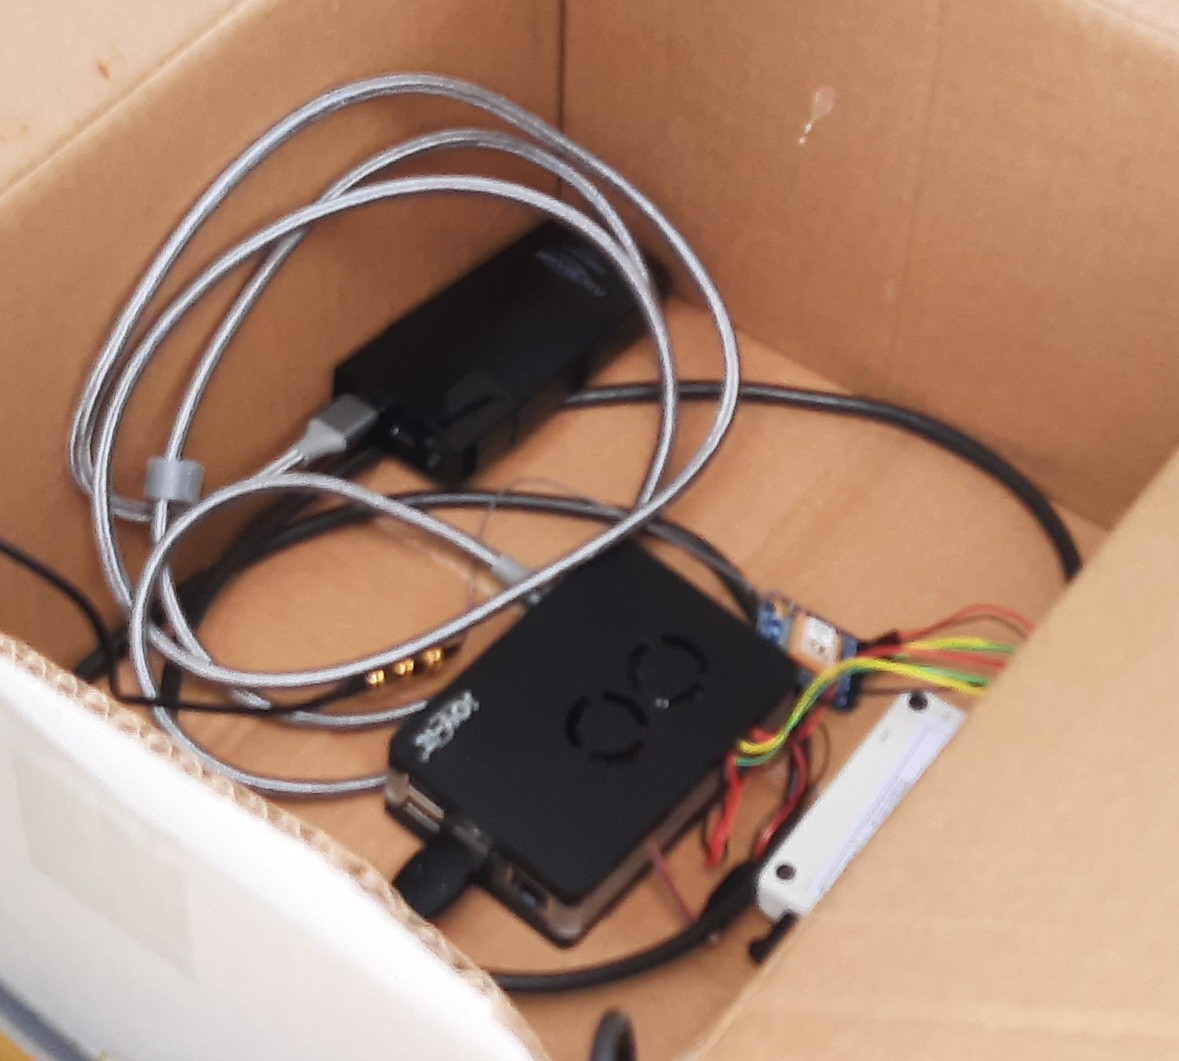
\includegraphics[width=.4\linewidth]{rtexps-pics/transmitter.jpg}
  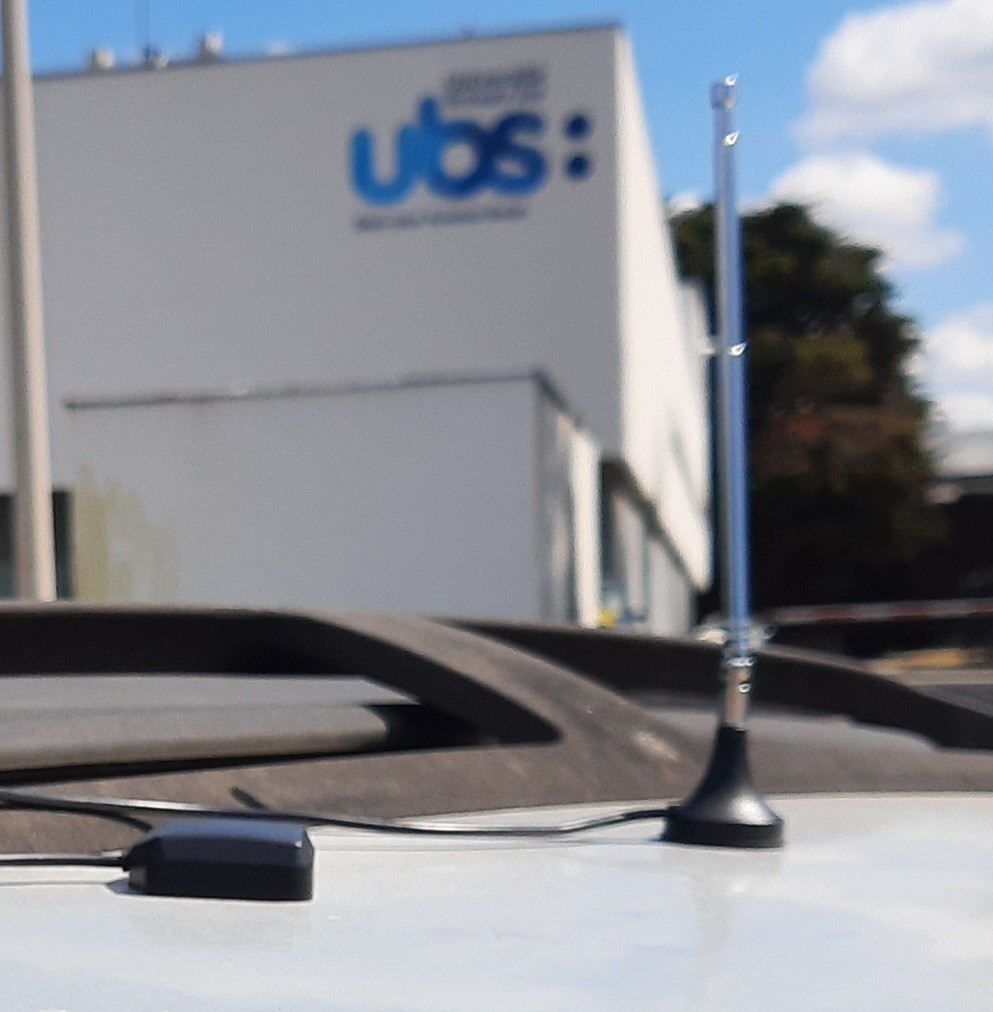
\includegraphics[width=.4\linewidth]{rtexps-pics/trans_antenna.jpg}
  \includegraphics[width=.4\linewidth]{rtexps-pics/receiver.png}
\end{frame}

\subsection{En mer}

\begin{frame}{\subsecname}
  \begin{center}
    \textcolor{RoyalBlue}{TODO}
  \end{center}
\end{frame}

\end{document}
